% SEC 3.1
\section{Introduction to Determinants}
\name

\begin{boxme}
	Given a matrix $A$, we define a submatrix, $A_{ij}$, by deleting the $i$th row and $j$th column. \par
	
	\textbf{Example:} Given $A$ below, you get $A_{23}$ by deleting the 2nd row and 3rd column from $A$.
	\begin{align*}
	A = \begin{tikzpicture}[baseline=-0.5ex]%\usetikzlibrary{arrows,matrix,positioning}
	\matrix[matrix of math nodes, matrix anchor=east,
	left delimiter={[},right delimiter={]},
	every odd column/.style={anchor=base east},
	every even column/.style={anchor=base east},
	column 3/.style={color=red},
	row 2/.style={color=red},
	ampersand replacement=\&
	] (A) at (0,0)
	{
		3 \& 0 \&  3  \\
		3 \& 4 \&  2  \\
		0 \& 5 \& -1  \\
	};
	\draw[color=red] (A-2-1.north west) rectangle (A-2-3.south east);
	\draw[color=red] (A-1-2.north east) rectangle (A-3-3.south east);
	\end{tikzpicture}
	\quad
	&\xrightarrow[\text{\& 3rd Column}]{\text{Delete 2nd Row}}
	\quad
	A_{23} = \begin{bmatrix} 3&0 \\ 0&5 \end{bmatrix}
	\end{align*}
\end{boxme}

\begin{exercise} % 3.1.5
	Given $A=\begin{bmatrix}6&7&-5\\2&0&4\\5&2&3\end{bmatrix}$, determine the following.
	\begin{multicols}{3}
		\begin{enumerate}[(a)]
			\item $\det A_{11}$
			\item $\det A_{12}$
			\item $\det A_{13}$
		\end{enumerate}
	\end{multicols}
\end{exercise}
\vfill

\begin{boxme}
	\vspace{-1em}
	\begin{multicols}{2}
		The $(i,j)$-cofactor of $A$ is defined as.
		\begin{align*}
		C_{ij} &= (-1)^{i+j}\det A_{ij}
		\end{align*}
		\textbf{Example:} (uses $A_{23}$ from previous example)
		\begin{align*}
		C_{23} &= (-1)^{2+3}\det A_{23} \\
		&= (-1)^5\begin{vmatrix} 3&0 \\ 0&5 \end{vmatrix} \\
		&= (-1)(3\cdot 5 - 0) = -15
		\end{align*}
		
		\columnbreak
		
		The factor $(-1)^{i+j}$ determines the following pattern of signs:
		$$\begin{bmatrix}[c] +&-&+&\cdots \\ -&+&-& \\ +&-&+& \\ \vdots&&&\ddots \end{bmatrix}$$
	\end{multicols}
\end{boxme}
\begin{boxdef}
	For $n\geq 2$, the \textbf{determinant} of an $n\times n$ matrix $A=[a_{ij}]$ is the sum of $n$ terms of the form $\pm a_{1j}\det A_{1j}$, with plus and minus signs alternating, where the entries $a_{11},a_{12},\ldots,a_{1n}$ are from the first row of $A$. 
	\begin{align*}
	\det A &= a_{11}\det A_{11} - a_{12}\det A_{12} + \cdots + (-1)^{1+n}a_{1n}\det A_{1n} \\
	&= \sum_{j=1}^n(-1)^{1+j}a_{1j}\det A_{1j}
	\end{align*}
\end{boxdef}
\begin{exercise} % 3.1.5
	Using Exercise 1 and the above definition, compute the determinant of $A=\begin{bmatrix}6&7&-5\\2&0&4\\5&2&3\end{bmatrix}$.
	\vspace{-1ex}
	\begin{align*}
	\det A &= a_{11}\det A_{11} - a_{12}\det A_{12} + \cdots + (-1)^{1+n}a_{1n}\det A_{1n} \\
	&= (6)\det A_{11} - (7)\det A_{12} + (-5)\det A_{13} \\[1em]
	&=
	\end{align*}
\end{exercise}
\vfill


\newpage

\begin{boxthm}
	\textbf{Theorem 3.1.} \\
	The determinant of a $n\times n$ matrix $A$ can be computed by a cofactor expansion across any row or down any column. The expansion across the $i$th row using the cofactors $C_{ij} = (-1)^{i+j}\det A_{ij}$ is
	$$ \det A = a_{i1}C_{i1} + a_{i2}C_{i2} + \cdots + a_{in}C_{in}. $$
	The cofactor expansion down the $j$th column is
	$$ \det A = a_{1j}C_{1j} + a_{2j}C_{2j} + \cdots + a_{nj}C_{nj}. $$
\end{boxthm}

\begin{exercise} % 3.1.9
	Compute the determinant by cofactor expansion. At each step, try to choose a row or column that involves the least amount of computation. \\
	
	$\begin{vmatrix}1&6&3&9\\0&7&0&3\\0&2&0&1\\4&-7&0&7\end{vmatrix}$
\end{exercise}
\vfill


\begin{boxthm}
	\textbf{Theorem 3.2.} \\
	If $A$ is a triangular matrix, then $\det A$ is the product of the entries on the main diagonal of $A$.
\end{boxthm}
\begin{exercise} % 3.1.
	Compute the following determinants.
	\begin{multicols}{3}
%		\pgfmathsetseed{101}
%	\begin{enumerate}[(a)]
%		\item 	$\begin{vmatrix}
%				\Rand&\Rand&\Rand\\
%				0&\Rand&\Rand\\
%				0&0&\Rand
%				\end{vmatrix}$
%		\item 	$\begin{vmatrix}
%				\Rand&-\Rand&\Rand&\Rand\\
%				0&-\Rand&\Rand&-\Rand\\
%				0&0&\Rand&\Rand\\
%				0&0&0&-\Rand
%				\end{vmatrix}$
%		\item	$\begin{vmatrix}
%				\Rand&\Rand&\Rand&\Rand&\Rand&\Rand\\
%				0&\Rand&\Rand&\Rand&\Rand&\Rand\\
%				0&0&\Rand&\Rand&\Rand&\Rand\\
%				0&0&0&\Rand&\Rand&\Rand\\
%				0&0&0&0&\Rand&\Rand\\
%				0&0&0&0&0&0
%				\end{vmatrix}$
%	\end{enumerate}
	\begin{enumerate}[(a)]
		\item
			$\begin{vmatrix}
			5&1&3\\
			0&3&3\\
			0&0&2
			\end{vmatrix}$
		\item 
			$\begin{vmatrix}
			3&-1&7& 5\\
			0&-3&2&-1\\
			0& 0&4& 7\\
			0& 0&0&-2
			\end{vmatrix}$
		\item
			$\begin{vmatrix}
			4&7&4&6&1&6\\
			0&1&6&4&4&1\\
			0&0&5&3&1&4\\
			0&0&0&1&4&1\\
			0&0&0&0&4&5\\
			0&0&0&0&0&0
			\end{vmatrix}$
	\end{enumerate}
	\end{multicols}
\end{exercise}
\vspace{1in}

\newpage

\section{Properties of Determinants}
\name

Read the Properties of Determinants Section outline from a different book and answer the following questions.  This reading assignment is due Wednesday, February 26, 2020 at the beginning of class.
\begin{boxthm}
	\textbf{Theorem 3.3.} \\
	Let $A$ be a square matrix.
	\begin{enumerate}[(a)]
		\item If a multiple of one row of $A$ is added to another row to produce $B$, then $\det B = \det A$.
		\item If two rows of $A$ are interchanged to produce $B$, then $\det B = -\det A$.
		\item If one row of $A$ is multiplied by $k$ to produce $B$, then $\det B = k\det A$.
	\end{enumerate}
\end{boxthm}

\begin{exercise} % 3.2.9
	Find the determinant of $A=\begin{bmatrix}1&-1&-3&0\\0&1&5&4\\-1&0&5&3\\3&-3&-2&3\end{bmatrix}$ by row reducing to a matrix of row echelon form.
\end{exercise}
\vfill

\begin{boxthm}
	\textbf{Theorem 3.4.} \\
	Let $A$ be a square matrix. $A$ is invertible if and only if $\det A \ne 0$.
\end{boxthm}

\begin{exercise}
Does the matrix, $A$, from the previous exercise have an inverse? Why or why not?
\end{exercise}

\vspace{2cm}

\newpage

\begin{boxthm}
	\textbf{Theorem 3.5.} \\
	If $A$ is a square matrix, then $\det A = \det A^T$.
\end{boxthm}

\begin{boxthm}
	\textbf{Theorem 3.6.} \\
	If $A$ and $B$ are both $n \times n$ matrices, then $\det AB = \det A \det B$.
\end{boxthm}

\begin{exercise}
Suppose $A$ and $B$ are both $3 \times 3$ matrices where $\det A = 2$ and $\det B = -3$. Use the theorems from both sides to determine each of the following:

\begin{enumerate}[(a)]

\item $\det AB$

\vfill

\item $\det A^T$

\vfill

\item $\det 5A$

\vfill

\item $\det B^{-1}$

\vfill

\item $\det A^3$

\vfill

\end{enumerate}

\end{exercise}

\newpage

\section{Cramer's Rule and Volume}
\name

\begin{boxthm}
	\textbf{Theorem 3.7: Cramer's Rule.} \\
	Let $A$ be an $n \times n$ invertible matrix. For any $\vect{b} \in \mathbb{R}^n$, the unique solution $\vect{x}$ of $A\vect{x}=\vect{b}$ has entries given by $$x_i = \frac{\det A_i(\vect{b})}{\det A}, \hspace{1cm} i = 1,2,...,n.$$
\end{boxthm}

\begin{exercise}
Consider the following system:

\[\systeme[x_1,x_2]{
	 5x_1	+	7x_2	= 3,
	2x_1	+	4x_2	= 1
	}
\]

\begin{enumerate}[(a)]

\item Rewrite the system in the form $A\vect{x}=\vect{b}$.
\vfill

\item Verify that $\det A \ne 0$, so that Cramer's Rule will apply.
\vfill

\item Solve the system using Cramer's Rule.
\vfill
\vfill
\vfill

\end{enumerate}
\end{exercise}

\newpage

\begin{boxthm}
	\textbf{Theorem 3.9.} \\
	If $A$ is a $2 \times 2$ matrix, the area of the parallelogram determined by by the columns of $A$ is $|\det A|$. If $A$ is a $3 \times 3$ matrix, the volume of the parallelepiped determined by the columns of $A$ is $|\det A|$.
\end{boxthm}

\begin{boxthm}
	\textbf{Theorem 3.10.} \\
	Let $T: \mathbb{R}^2 \rightarrow \mathbb{R}^2$ be a linear transformation determined by $2 \times 2$ matrix $A$. If $S$ is a parallelogram in $\mathbb{R}^2$, then $$\{ \text{area of } T(S)\} = |\det A| \cdot \{ \text{area of } S \}.$$
	
	Alternatively, let $T: \mathbb{R}^3 \rightarrow \mathbb{R}^3$ be a linear transformation determined by $3 \times 3$ matrix $A$. If $S$ is a parallelepiped in $\mathbb{R}^3$, then $$\{ \text{volume of } T(S)\} = |\det A| \cdot \{ \text{volume of } S \}.$$
\end{boxthm}

\begin{exercise}

Let $S$ be the parallelogram determined by the vectors $\vect{b_1} = \begin{bmatrix}2\\1\end{bmatrix}$ and $\vect{b_2} = \begin{bmatrix}1\\3\end{bmatrix}$.

\begin{enumerate}[(a)]

\item Shade in $S$ in the picture below. Then, use a determinant to find the area of $S$.

\hfill 	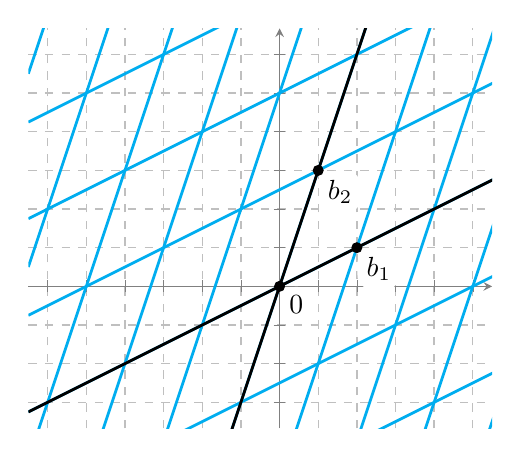
\begin{tikzpicture}[scale=1]
	% Set u and v
	\pgfmathsetmacro{\ux}{2}
	\pgfmathsetmacro{\uy}{1}
	\pgfmathsetmacro{\vx}{1}
	\pgfmathsetmacro{\vy}{3}
	\pgfmathsetmacro{\xcoor}{-4}
	\pgfmathsetmacro{\ycoor}{3}
	% Begin Axis
	\begin{axis}[axis x line=center, axis y line=middle,
	xmin=-6.5, xmax=5.5,
	ymin=-3.5, ymax=6.5,
	xtick={-6,...,5}, ytick={-3,...,7},
	xticklabels={,,}, yticklabels={,,},
	scale only axis, axis equal, height=2in,
	gray,
	grid=major, grid style={line width=.5pt, draw=gray!50, dashed}]
	% Plot alternate coordinate system
	\foreach \yi in {-10,...,10}{
		\addplot[-, cyan, line width=1pt, domain=-6.5:6.5] {(\uy/\ux)*(x-\yi*\vx)+\vy*\yi};
	}
	\foreach \xi in {-10,...,10}{
		\addplot[-, cyan, line width=1pt, domain=-6.5:6.5] {(\vy/\vx)*(x-\xi*\ux)+\uy*\xi};
	}
	\addplot[-, black, line width=1pt, domain=-6.5:6.5] {(\uy/\ux)*x};
	\addplot[-, black, line width=1pt, domain=-6.5:6.5] {(\vy/\vx)*x};
	% Plot vectors
	\fill[black] (0,0) circle (2pt) node[below right, fill=white, rounded corners=0.2cm] {$\vect{0}$};
	\fill[black] (\ux,\uy) circle (2pt) node[below right, fill=white, rounded corners=0.2cm] {$\vect{b}_1$};
	\fill[black] (\vx,\vy) circle (2pt) node[below right, fill=white, rounded corners=0.2cm] {$\vect{b}_2$};
	%\fill[black] (\xcoor,\ycoor) circle (2pt) node[below right, fill=white, rounded corners=0.2cm] {$\vect{x}$};
	\end{axis}
	\end{tikzpicture}

\item Find the area of the image of $S$ under the mapping $\vect{x} \rightarrow A\vect{x}$ where $A =\begin{bmatrix}5&-1\\2&5\end{bmatrix}$.
\vfill
\vfill

\end{enumerate}

\end{exercise}

% MISSING SECTIONS 3.2-3.3, 4.1-4.2
% Missed a few sections when Romy was born. (3.2, 3.3, 4.1, 4.2)
% SEC 3.3
%\section{Cramer's Rule, Volume, and Linear Transformations}


\newpage

